Model standardowy – teoria fizyki cząstek podstawowych, zwanych też cząstkami elementarnymi, które są podstawowymi składnikami każdej materii (rys.~\ref{standard_model}). Opisuje trzy z czterech (z wyjątkiem grawitacji) oddziaływań podstawowych: elektromagnetyczne, słabe i silne. Sformułowana jest w języku matematyki, opisując relacjami matematycznymi zależności między elementami tej teorii. Opiera się na koncepcji pola Yanga-Millsa (pole rządzące oddziaływaniem wszystkich znanych cząstek we wszechświecie).

\begin{figure} [H]
	\centering
	\begin{subfigure}{.99\textwidth}
		\centering
		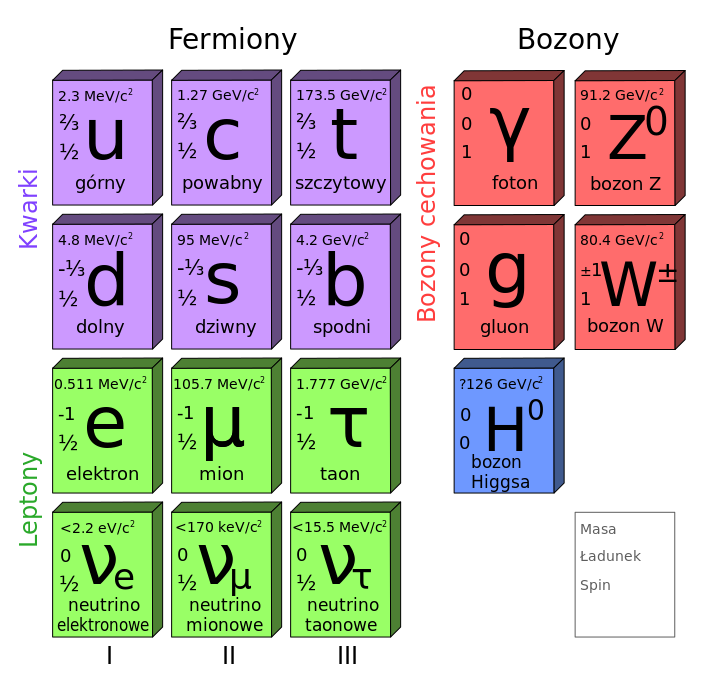
\includegraphics[width=0.7\linewidth]{generalIssues/Figures/standard_model.png}
	\end{subfigure}
	\caption{Cząstki elementarne według Modelu Standardowego.}
	\label{standard_model}
\end{figure}

Fermiony są podstawowymi elementami budującymi materię. Materię trwałą, która nas otacza, tworzą następujące cząstki: elektron, kwark górny (u) oraz kwark dolny (d) np.  dwa kwarki górne i jeden dolny (uud) tworzą proton. Kwarki mają kolor i zapach (są to nazwy nadane umownie pewnym liczbom kwantowym). Do tej grupy cząstek należy też neutrino elektronowe, a grupa ta tworzy pierwszą generację. Kolejne dwie generacje zawieraja po cztery cząstki odpowiadające cząstkom z pierwszej generacji (lecz o różnej masie).

Bozony cechowania przenoszą oddziaływania:
\begin{itemize}
	\item elektromagnetyczne - przenoszone jest przez foton. Oddziaływanie to odbywa się poprzez wytworzenie lub pochłonięcie fotonu.
	\item słabe - powodujące między innymi rozpady beta, przenoszone jest przez bozony $ W^+ $ i $ W^- $ oraz $ Z^0 $.
	\item silne - łączące kwarki w hadrony, przenoszone jest przez osiem rodzajów gluonów, sposób oddziaływania (rodzaj gluonu) oznaczany jest właściwością nazywaną kolorem gluonu. Hadrony złożone są z kwarków występujących przeważnie trójkami (trzy kwarki lub trzy antykwarki tworzą bariony - spin połówkowy, liczba barionowa = 1) lub parami (pary kwark i antykwark tworzą mezony - spin całkowity, liczba barionowa = 0). Właściwością hadronów jest również ich całkowity ładunek elektryczny.
\end{itemize}

Bozon Higgsa (istnienie którego udało się potwierdzić doświadczalnie w 2012 roku) oddziałując z innymi cząstkami nadaje im masę (głównie dotyczy nadawania masy elektronowi, nie dotyczy nadawania masy protonowi i neutronowi, których masa wynika z innego mechanizmu).

Model standardowy jest potwierdzony doświadczalnie, lecz nie jest w pełni satysfakcjonujący z teoretycznego punktu widzenia:

\begin{itemize}
	\item Ma 19 swobodnych parametrów (np. masy cząstek), które należy wyznaczyć doświadczalnie, gdyż teoria nie wyjaśnia ich wartości.
	\item Obliczenia masy Wszechświata nie zgadzają się z obserwowaną ilością materii we Wszechświecie, brakującą materię nazywa się ciemną materią.
	\item W podstawowej wersji nie uwzględnia mas neutrin.
\end{itemize}

Protony i neutrony związane oddziaływaniem silnym (za pośrednictwem mezonów $ \mu $) tworzą jądra atomowe. Protony odpychają się elektrostatycznie, jednak jądro utrzymywane jest w całości przez oddziaływanie silne. Działa ono tylko na niewielką odległość, dlatego jądra zbyt duże i masywne stają się nietrwałe, co prowadzi do samorzutnego ich rozpadu. Liczba protonów w jądrze atomowym to liczba atomowa, a suma liczb protonów i neutronów to liczba masowa.

Obiekt fizyczny złożony z jądra atomowego i znajdujących się w otoczeniu jądra, związanych z nim oddziaływaniem elektromagnetycznym (siłą elektrostatyczną), elektronów to atom. 

Atomy mogą łączyć się w cząsteczki, których względną trwałość zapewniają wiązania chemiczne.

Atomy mogą łączyć się w cząsteczki, których względną trwałość zapewniają wiązania chemiczne. Wiązania chemiczne powstają dzięki wymianie elektronów między atomami, która może odbywać się na dwa sposoby:
\begin{itemize}
	\item kowalencyjny – polegający na uwspólnianiu par elektronów przez dwa lub więcej atomów,
	\item jonowy – polegający na trwałym przeniesieniu elektronów z jednego atomu na drugi, w którego wyniku na jednym z atomów tworzy się całkowity ładunek ujemny, a na drugim dodatni; w efekcie powstaje para jonowa, która jest związana z sobą zwykłymi oddziaływaniami elektrostatycznymi.
\end{itemize}